%%%%%%%%%%%%%%%%%%%%%%%%%%%%%%%%%%%%%%%%%%%%%%%%%%%%%%%%%%%%%
%% Begin exercise %%
%%%%%%%%%%%%%%%%%%%%%%%%%%%%%%%%%%%%%%%%%%%%%%%%%%%%%%%%%%%%%
\ex{Parasitics, ringing and snubbers}

%%%%%%%%%%%%%%%%%%%%%%%%%%%%%%%%%%%%%%%%%%%%%%%%%%%%%%%%%%%%%
%% Task 1 %%
%%%%%%%%%%%%%%%%%%%%%%%%%%%%%%%%%%%%%%%%%%%%%%%%%%%%%%%%%%%%%

\task{Loop inductance of a power loop}

The power loop of a GaN half-bridge runs on the top layer L1 of a 4-layer board: the copper from the input capacitors through both transistors is $w=\SI{4}{\milli\metre}$ wide and $l=\SI{10}{\milli\metre}$ long (\autoref{fig:ex03_loop}). The return current flows in a solid plane, either on L2 at $h=\SI{0.1}{\milli\metre}$ or on L4 at $h=\SI{1.5}{\milli\metre}$.

%%%%%%%%%%%%%%%%%%%%%%%%%%%%%%%%%%%%%%%%%%%%%%%%%%%%%%%%%%%%%%%%%%%%%%%%%%
% Cross-section of the power-loop copper over its return plane (Exercise 03, Task 1)
%%%%%%%%%%%%%%%%%%%%%%%%%%%%%%%%%%%%%%%%%%%%%%%%%%%%%%%%%%%%%%%%%%%%%%%%%%

\begin{figure}[htb]
	\begin{center}
		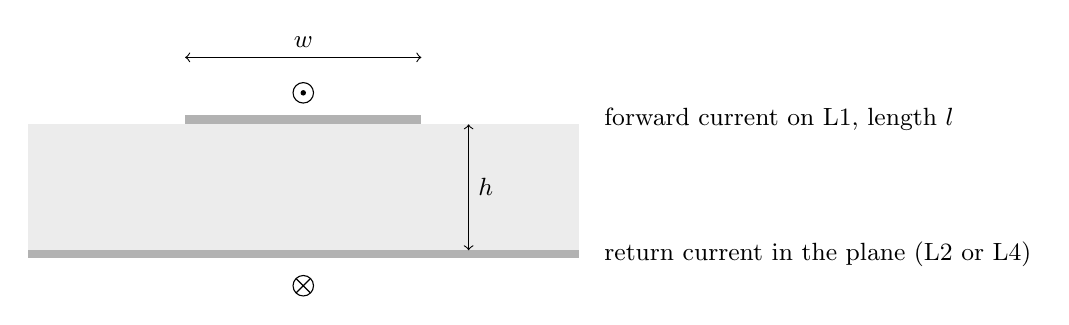
\begin{tikzpicture}[font=\small]
			% laminate, return plane and forward copper (not to scale)
			\fill[gray!15] (0,0) rectangle (7,1.6);
			\fill[gray!60] (0,-0.1) rectangle (7,0);
			\fill[gray!60] (2.0,1.6) rectangle (5.0,1.72);
			% current directions
			\draw (3.5,2.0) circle (0.13); \fill (3.5,2.0) circle (0.035);
			\draw (3.5,-0.45) circle (0.13);
			\draw (3.5,-0.45) ++(-0.09,-0.09) -- ++(0.18,0.18) ++(0,-0.18) -- ++(-0.18,0.18);
			% dimensions
			\draw[<->] (2.0,2.45) -- (5.0,2.45) node[midway, above] {$w$};
			\draw[<->] (5.6,0) -- (5.6,1.6) node[midway, right] {$h$};
			% labels
			\node[anchor=west] at (7.2,1.66) {forward current on L1, length $l$};
			\node[anchor=west] at (7.2,-0.05) {return current in the plane (L2 or L4)};
		\end{tikzpicture}
	\end{center}
	\caption{Cross-section of the power loop: forward copper of width $w$ over a solid return plane at the distance $h$ (not to scale).}
	\label{fig:ex03_loop}
\end{figure}


\subtask{Estimate the loop inductance for both return layers with the parallel-plane formula $L\approx\mu_0hl/w$.}

\begin{solutionblock}
	\begin{equation}
		L_\mathrm{L2} \approx \mu_0\frac{hl}{w} = \SI{1.257}{\nano\henry\per\milli\metre}\cdot\frac{\SI{0.1}{\milli\metre}\cdot\SI{10}{\milli\metre}}{\SI{4}{\milli\metre}} = \SI{0.31}{\nano\henry},\qquad
		L_\mathrm{L4} \approx \SI{4.7}{\nano\henry}.
	\end{equation}
\end{solutionblock}

\subtask{For a strip of width $w$ over a wide plane at the distance $h$ the inductance per length is $L'=Z_0/c_0$, where $Z_0$ is the characteristic impedance of the strip in air ($c_0=\SI{3 \cdot 10^{8}}{\metre\per\second}$). For $w/h\geq1$ (Hammerstad):
\begin{equation*}
	Z_0=\frac{\SI{376.7}{\ohm}}{w/h+1.393+0.667\ln(w/h+1.444)}.
\end{equation*}
Recalculate both cases and explain the difference to the parallel-plane formula.}

\begin{solutionblock}
	L2: $w/h=40$, $Z_0=\SI{8.59}{\ohm}$, $L'=\SI{28.6}{\pico\henry\per\milli\metre}$, $L=\SI{0.29}{\nano\henry}$, i.e.\ 9\,\% below the parallel-plane value.\\
	L4: $w/h=2.67$, $Z_0=\SI{75.3}{\ohm}$, $L'=\SI{0.251}{\nano\henry\per\milli\metre}$, $L=\SI{2.5}{\nano\henry}$, i.e.\ 47\,\% below the parallel-plane value.\\
	The parallel-plane formula assumes that the whole field is confined to the volume $w\cdot h\cdot l$. For $w\gg h$ this holds. For $w/h\approx3$ a large part of the field spreads beside the strip, the effective width is larger than $w$ and the formula overestimates the inductance. The inductance does not depend on the permittivity of the laminate.
\end{solutionblock}

\subtask{With the return on L4 the loop is closed by four vias at each end ($d=\SI{0.3}{\milli\metre}$, length $\SI{1.5}{\milli\metre}$). Estimate the partial inductance of one via and of four vias in parallel. Why is the second value optimistic?}

\begin{solutionblock}
	\begin{equation}
		L_\mathrm{p}\approx\SI{0.2}{\nano\henry\per\milli\metre}\cdot l\left[\ln\frac{4l}{d}-1\right] = \SI{0.2}{\nano\henry\per\milli\metre}\cdot\SI{1.5}{\milli\metre}\cdot(\ln 20-1) = \SI{0.60}{\nano\henry}.
	\end{equation}
	Four vias in parallel give $\SI{0.15}{\nano\henry}$ only if they do not couple. Vias that carry current in the same direction have a positive mutual inductance, so the parallel combination is larger. Interleaving them with vias of the opposite current direction reduces it instead.
\end{solutionblock}

\subtask{The example file \texttt{loop\_L2\_return.inp} (folder \texttt{code/ex03}) describes this loop for the field solver FastHenry, including vias and capacitor pad. It gives $\SI{0.48}{\nano\henry}$ with the return on L2 and $\SI{3.1}{\nano\henry}$ with the return on L4. Which change lowers the inductance of the L4 version most: doubling $w$, halving $l$, or moving the return to L2? Use the strip formula.}

\begin{solutionblock}
	Doubling $w$: $w/h=5.33$, $Z_0=\SI{47.1}{\ohm}$, $L=\SI{1.57}{\nano\henry}$ (factor 1.6 instead of 2, because the field beside the strip does not halve).\\
	Halving $l$: $L=\SI{1.26}{\nano\henry}$ (factor 2).\\
	Return on L2: $L=\SI{0.29}{\nano\henry}$ (factor 8.8).\\
	The distance between forward and return current is the most effective parameter. The field solver confirms the trend; its absolute values are higher because they include the vias, the capacitor pad and the current spreading in the plane.
\end{solutionblock}

%%%%%%%%%%%%%%%%%%%%%%%%%%%%%%%%%%%%%%%%%%%%%%%%%%%%%%%%%%%%%
%% Task 2 %%
%%%%%%%%%%%%%%%%%%%%%%%%%%%%%%%%%%%%%%%%%%%%%%%%%%%%%%%%%%%%%

\task{Loop inductance from a measured ring}

After the turn-on of the high-side switch, the switch-node voltage of a $\SI{48}{\volt}$ GaN half-bridge rings at $f_\mathrm{r0}=\SI{200}{\mega\hertz}$. A $\SI{330}{\pico\farad}$ C0G capacitor is soldered directly across the low-side switch; the ringing frequency drops to $f_\mathrm{r1}=\SI{141}{\mega\hertz}$. The datasheet gives $C_\mathrm{oss}=\SI{300}{\pico\farad}$ at $\SI{48}{\volt}$.

\subtask{Derive the total capacitance $C_\mathrm{par}$ across the low-side switch and the loop inductance from the two measurements. Calculate $Z_0$.}

\begin{solutionblock}
	With $f_\mathrm{r0}=1/(2\pi\sqrt{LC_\mathrm{par}})$ and $f_\mathrm{r1}=1/(2\pi\sqrt{L(C_\mathrm{par}+C_\mathrm{add})})$:
	\begin{equation}
		\left(\frac{f_\mathrm{r0}}{f_\mathrm{r1}}\right)^2 = \frac{C_\mathrm{par}+C_\mathrm{add}}{C_\mathrm{par}}\ \Rightarrow\
		C_\mathrm{par} = \frac{C_\mathrm{add}}{(f_\mathrm{r0}/f_\mathrm{r1})^2-1} = \frac{\SI{330}{\pico\farad}}{2.012-1} = \SI{326}{\pico\farad},
	\end{equation}
	\begin{equation}
		L_\mathrm{loop} = \frac{1}{(2\pi f_\mathrm{r0})^2C_\mathrm{par}} = \SI{1.94}{\nano\henry},\qquad
		Z_0 = \sqrt{\frac{L_\mathrm{loop}}{C_\mathrm{par}}} = \SI{2.44}{\ohm}.
	\end{equation}
\end{solutionblock}

\subtask{$C_\mathrm{par}$ is larger than $C_\mathrm{oss}$. Name possible contributions to the difference. Why must the added capacitor be small and mounted directly across the switch?}

\begin{solutionblock}
	The difference of about $\SI{26}{\pico\farad}$ comes from the switch-node copper over the planes, the winding capacitance of the output inductor, the probe and the tolerance of $C_\mathrm{oss}$.\\
	The added capacitor must carry the ringing current with its own small inductance. An ESL of $\SI{0.4}{\nano\henry}$ makes a $\SI{330}{\pico\farad}$ capacitor appear as $C/(1-\omega^2L_\mathrm{ESL}C)=\SI{368}{\pico\farad}$ at $\SI{141}{\mega\hertz}$. The ring frequency then drops further and the method underestimates $C_\mathrm{par}$ by about 10\,\% (see notebook).
\end{solutionblock}

\subtask{At the turn-on of the high-side switch the switch-node voltage rises linearly within $t_\mathrm{r}$. For an undamped $LC$ circuit the remaining oscillation then has the amplitude $V_\mathrm{DC}\,|\sin x|/x$ with $x=\pi f_\mathrm{r0}t_\mathrm{r}$. Calculate the peak voltage of the low-side switch for $t_\mathrm{r}=1$, 2.5 and $\SI{5}{\nano\second}$.}

\begin{solutionblock}
	\begin{solutiontable}[ht]
		\centering
		\begin{tabular}{lccc}
			\toprule
			$t_\mathrm{r}$                    & $\SI{1}{\nano\second}$ & $\SI{2.5}{\nano\second}$ & $\SI{5}{\nano\second}$ \\
			\midrule
			$x=\pi f_\mathrm{r0}t_\mathrm{r}$ & 0.63                   & 1.57                     & 3.14                   \\
			overshoot $V_\mathrm{DC}|\sin x|/x$ & $\SI{44.9}{\volt}$   & $\SI{30.6}{\volt}$       & $\SI{0}{\volt}$        \\
			peak voltage                      & $\SI{93}{\volt}$       & $\SI{79}{\volt}$         & $\SI{48}{\volt}$       \\
			\bottomrule
		\end{tabular}
		\caption{Turn-on overshoot without damping.}
		\label{stable:ex03_turnon}
	\end{solutiontable}
	An edge that lasts exactly one ringing period ($T_\mathrm{r}=\SI{5}{\nano\second}$) excites no oscillation in this ideal model. In practice the damping and the nonlinear $C_\mathrm{oss}$ reduce the peaks, but a $\SI{100}{\volt}$ device has no margin with the fast edge.
\end{solutionblock}

%%%%%%%%%%%%%%%%%%%%%%%%%%%%%%%%%%%%%%%%%%%%%%%%%%%%%%%%%%%%%
%% Task 3 %%
%%%%%%%%%%%%%%%%%%%%%%%%%%%%%%%%%%%%%%%%%%%%%%%%%%%%%%%%%%%%%

\task{Overshoot at turn-off}

At the turn-off of the high-side switch the load current $I$ has already been taken over by the low-side switch, which clamps the switch node. The channel current of the high-side switch falls linearly from $I$ to zero within $t_\mathrm{f}$ (\autoref{fig:ex03_turnoff}). Use $L_\mathrm{loop}=\SI{1.94}{\nano\henry}$, $C=\SI{326}{\pico\farad}$ and $I=\SI{10}{\ampere}$ from Task 3.2; the circuit is lossless.

%%%%%%%%%%%%%%%%%%%%%%%%%%%%%%%%%%%%%%%%%%%%%%%%%%%%%%%%%%%%%%%%%%%%%%%%%%
% Turn-off model with loop inductance (Exercise 03, Task 3)
%%%%%%%%%%%%%%%%%%%%%%%%%%%%%%%%%%%%%%%%%%%%%%%%%%%%%%%%%%%%%%%%%%%%%%%%%%

\begin{figure}[htb]
	\begin{center}
		\begin{circuitikz}
			\draw (0,0) to[V, l=$V_\mathrm{DC}$] (0,3) to[L, l=$L_\mathrm{loop}$, i>^=$i_L$] (3,3) -- (5,3);
			\draw (3,3) to[I, l_=$i_\mathrm{ch}(t)$] (3,0);
			\draw (5,3) to[C, l=$C$] (5,0);
			\draw (0,0) -- (5,0);
			\draw (3,3) node[circ]{} (3,0) node[circ]{} (5,3) node[circ]{};
			\draw (5,3) node[anchor=south]{A};
		\end{circuitikz}
	\end{center}
	\caption{Turn-off of the high-side switch after the low-side switch has taken over the load current (shown as a short circuit): channel current $i_\mathrm{ch}(t)$, capacitance $C$ across the switch and loop inductance $L_\mathrm{loop}$; $v_\mathrm{DS}=v_\mathrm{A}$.}
	\label{fig:ex03_turnoff}
\end{figure}


\subtask{Show that the overshoot $u=v_\mathrm{DS}-V_\mathrm{DC}$ obeys $\ddot{u}+\omega_0^2u=-\frac{1}{C}\frac{\mathrm{d}i_\mathrm{ch}}{\mathrm{d}t}$ with $\omega_0=1/\sqrt{L_\mathrm{loop}C}$.}

\begin{solutionblock}
	Mesh and node equations: $L_\mathrm{loop}\,\mathrm{d}i_L/\mathrm{d}t=V_\mathrm{DC}-v_\mathrm{DS}=-u$ and $C\,\mathrm{d}u/\mathrm{d}t=i_L-i_\mathrm{ch}$. Differentiating the second equation and inserting the first:
	\begin{equation}
		C\ddot{u} = -\frac{u}{L_\mathrm{loop}} - \frac{\mathrm{d}i_\mathrm{ch}}{\mathrm{d}t}
		\ \Rightarrow\ \ddot{u}+\omega_0^2u = -\frac{1}{C}\frac{\mathrm{d}i_\mathrm{ch}}{\mathrm{d}t}.
	\end{equation}
\end{solutionblock}

\subtask{Solve the equation for the linear current fall with $u(0)=0$ and $\dot{u}(0)=0$. Give $u(t)$ during the fall and the amplitude of the oscillation after it.}

\begin{solutionblock}
	During the fall $\mathrm{d}i_\mathrm{ch}/\mathrm{d}t=-I/t_\mathrm{f}$ is constant:
	\begin{equation}
		u(t) = \frac{I}{\omega_0^2Ct_\mathrm{f}}\left(1-\cos\omega_0t\right) = \frac{L_\mathrm{loop}I}{t_\mathrm{f}}\left(1-\cos\omega_0t\right),\qquad 0\leq t\leq t_\mathrm{f}.
	\end{equation}
	For $t>t_\mathrm{f}$ the circuit oscillates freely. From $u(t_\mathrm{f})$ and $\dot{u}(t_\mathrm{f})$ the amplitude is
	\begin{equation}
		\hat{u} = \frac{L_\mathrm{loop}I}{t_\mathrm{f}}\sqrt{(1-\cos\omega_0t_\mathrm{f})^2+\sin^2\omega_0t_\mathrm{f}} = \frac{2L_\mathrm{loop}I}{t_\mathrm{f}}\left|\sin\frac{\omega_0t_\mathrm{f}}{2}\right|.
	\end{equation}
\end{solutionblock}

\subtask{Show that the amplitude approaches $I\,Z_0$ for $t_\mathrm{f}\rightarrow0$. Evaluate the maximum overshoot for $t_\mathrm{f}=\SI{0.5}{\nano\second}$ and $t_\mathrm{f}=\SI{4}{\nano\second}$ and compare it with $L_\mathrm{loop}I/t_\mathrm{f}$ and $I\,Z_0$.}

\begin{solutionblock}
	For small $t_\mathrm{f}$, $|\sin(\omega_0t_\mathrm{f}/2)|\approx\omega_0t_\mathrm{f}/2$ and $\hat{u}\rightarrow L_\mathrm{loop}I\omega_0=I\sqrt{L_\mathrm{loop}/C}=I\,Z_0=\SI{24.4}{\volt}$. With $\omega_0=\SI{1.257 \cdot 10^{9}}{\per\second}$ ($T_\mathrm{r}=\SI{5}{\nano\second}$):
	\begin{solutiontable}[ht]
		\centering
		\begin{tabular}{lcc}
			\toprule
			$t_\mathrm{f}$                                & $\SI{0.5}{\nano\second}$ & $\SI{4}{\nano\second}$ \\
			\midrule
			$L_\mathrm{loop}I/t_\mathrm{f}$               & $\SI{38.8}{\volt}$       & $\SI{4.9}{\volt}$      \\
			maximum of $u$ during the fall                & $\SI{7.4}{\volt}$        & $\SI{9.7}{\volt}$      \\
			amplitude $\hat{u}$ after the fall            & $\SI{24.0}{\volt}$       & $\SI{5.7}{\volt}$      \\
			\bottomrule
		\end{tabular}
		\caption{Turn-off overshoot without damping, $I\,Z_0=\SI{24.4}{\volt}$.}
		\label{stable:ex03_turnoff}
	\end{solutiontable}
	For the fast fall the overshoot is close to $I\,Z_0$ and $L\,\mathrm{d}i/\mathrm{d}t$ overestimates it by a factor of 1.6. For the slow fall the undamped model gives up to $2L_\mathrm{loop}I/t_\mathrm{f}$; with damping the voltage settles near $L_\mathrm{loop}I/t_\mathrm{f}$. $I\,Z_0$ is an upper bound for any monotonic current fall in the lossless circuit.
\end{solutionblock}

%%%%%%%%%%%%%%%%%%%%%%%%%%%%%%%%%%%%%%%%%%%%%%%%%%%%%%%%%%%%%
%% Task 4 %%
%%%%%%%%%%%%%%%%%%%%%%%%%%%%%%%%%%%%%%%%%%%%%%%%%%%%%%%%%%%%%

\task{RC snubber}

The ring of Task 3.2 shall be damped by an RC snubber across the low-side switch (\autoref{fig:ex03_snubber}). The converter switches at $f_\mathrm{sw}=\SI{1}{\mega\hertz}$.

%%%%%%%%%%%%%%%%%%%%%%%%%%%%%%%%%%%%%%%%%%%%%%%%%%%%%%%%%%%%%%%%%%%%%%%%%%
% Ringing circuit with RC snubber (Exercise 03, Task 4)
%%%%%%%%%%%%%%%%%%%%%%%%%%%%%%%%%%%%%%%%%%%%%%%%%%%%%%%%%%%%%%%%%%%%%%%%%%

\begin{figure}[htb]
	\begin{center}
		\begin{circuitikz}
			\draw (0,0) to[V, l=$V_\mathrm{DC}$] (0,3) to[L, l=$L_\mathrm{loop}$] (3,3) -- (5,3);
			\draw (3,3) to[C, l=$C_\mathrm{par}$] (3,0);
			\draw (5,3) to[R, l=$R_\mathrm{s}$] (5,1.5) to[C, l=$C_\mathrm{s}$] (5,0);
			\draw (0,0) -- (5,0);
			\draw (3,3) node[circ]{} (3,0) node[circ]{};
		\end{circuitikz}
	\end{center}
	\caption{Ringing circuit of the switch that is off ($C_\mathrm{par}=C_\mathrm{oss}+$ layout) with an RC snubber $R_\mathrm{s}$, $C_\mathrm{s}$ across the switch.}
	\label{fig:ex03_snubber}
\end{figure}


\subtask{Choose $C_\mathrm{s}$ as the next E6 value above $3C_\mathrm{par}$ and $R_\mathrm{s}$ as the E12 value closest to $Z_0$.}

\begin{solutionblock}
	$3C_\mathrm{par}=\SI{978}{\pico\farad}$, so $C_\mathrm{s}=\SI{1}{\nano\farad}$; $Z_0=\SI{2.44}{\ohm}$, so $R_\mathrm{s}=\SI{2.2}{\ohm}$.
\end{solutionblock}

\subtask{With $n=C_\mathrm{s}/C_\mathrm{par}$, $r=R_\mathrm{s}/Z_0$ and $p=s/\omega_0$ the characteristic equation of the circuit is $rnp^3+(1+n)p^2+rnp+1=0$. Derive it. For the chosen values the dominant pair of roots gives the damping ratio $\zeta=0.51$ and the natural frequency $\SI{136}{\mega\hertz}$ (see notebook). Interpret the result.}

\begin{solutionblock}
	The node with $C_\mathrm{par}$ and the snubber branch has the admittance $Y=sC_\mathrm{par}+sC_\mathrm{s}/(1+sR_\mathrm{s}C_\mathrm{s})$. The natural frequencies follow from $1+sL_\mathrm{loop}Y=0$:
	\begin{equation}
		s^3L_\mathrm{loop}C_\mathrm{par}R_\mathrm{s}C_\mathrm{s}+s^2L_\mathrm{loop}(C_\mathrm{par}+C_\mathrm{s})+sR_\mathrm{s}C_\mathrm{s}+1=0.
	\end{equation}
	With $s=p\,\omega_0$, $\omega_0^2L_\mathrm{loop}C_\mathrm{par}=1$ and $\omega_0R_\mathrm{s}C_\mathrm{s}=rn$ this becomes $rnp^3+(1+n)p^2+rnp+1=0$.\\
	With $\zeta=0.51$ the amplitude drops to about 2.5\,\% within one period ($e^{-2\pi\zeta/\sqrt{1-\zeta^2}}$) instead of ringing for many periods. The natural frequency drops from $\SI{200}{\mega\hertz}$ to $\SI{136}{\mega\hertz}$ because $C_\mathrm{s}$ partly adds to $C_\mathrm{par}$; the damped oscillation has $\SI{117}{\mega\hertz}$. For $n=3.07$ the maximum damping, $\zeta=0.51$, is reached at $R_\mathrm{s}=0.93\,Z_0$, so the E12 value is close to the optimum.
\end{solutionblock}

\subtask{Estimate the loss of the snubber at $\SI{48}{\volt}$ and compare it with the energy $\frac12L_\mathrm{loop}I^2$ that the ring dissipates per period at $I=\SI{10}{\ampere}$. What do you recommend?}

\begin{solutionblock}
	At each switch-node edge $C_\mathrm{s}$ is charged or discharged through $R_\mathrm{s}$. For edges that are fast compared with $R_\mathrm{s}C_\mathrm{s}=\SI{2.2}{\nano\second}$, this costs $\frac12C_\mathrm{s}V^2=\SI{1.15}{\micro\joule}$ per edge in addition to the losses without snubber (the resistor also absorbs the ring energy, which would otherwise be dissipated elsewhere in the loop):
	\begin{equation}
		\SI{1.15}{\watt}\leq P_\mathrm{s}\leq C_\mathrm{s}V^2f_\mathrm{sw}=\SI{2.3}{\watt},
	\end{equation}
	depending on whether one or both edges are fast. The ring itself dissipates $\frac12L_\mathrm{loop}I^2f_\mathrm{sw}=\SI{0.1}{\watt}$.\\
	Recommendation: reduce $L_\mathrm{loop}$ by layout first (Task 3.1), which lowers $Z_0$ and the overshoot without loss. Use a smaller snubber capacitance only if the overshoot or the EMI spectrum still require it.
\end{solutionblock}

%%%%%%%%%%%%%%%%%%%%%%%%%%%%%%%%%%%%%%%%%%%%%%%%%%%%%%%%%%%%%
%% Task 5 %%
%%%%%%%%%%%%%%%%%%%%%%%%%%%%%%%%%%%%%%%%%%%%%%%%%%%%%%%%%%%%%

\task{Capacitive coupling of the switch node}

A $\SI{400}{\volt}$ half-bridge with 650\,V GaN transistors switches with $\mathrm{d}v/\mathrm{d}t=\SI{100}{\volt\per\nano\second}$ (edge time $\SI{4}{\nano\second}$) at $f_\mathrm{sw}=\SI{500}{\kilo\hertz}$. The high-side transistor is bottom-cooled: its source pad, which is the switch node, is mounted with an area of $\SI{48}{\milli\metre\squared}$ on a $\SI{0.25}{\milli\metre}$ thermal interface ($\varepsilon_\mathrm{r}=6$) on an earthed heat sink.

\subtask{Estimate the capacitance to the heat sink, the common-mode current during an edge and the charge per edge. Where does this current flow?}

\begin{solutionblock}
	\begin{equation}
		C=\varepsilon_0\varepsilon_\mathrm{r}\frac{A}{d}=\SI{8.854}{\pico\farad\per\metre}\cdot6\cdot\frac{\SI{48}{\milli\metre\squared}}{\SI{0.25}{\milli\metre}}=\SI{10.2}{\pico\farad},
	\end{equation}
	$i=C\,\mathrm{d}v/\mathrm{d}t=\SI{1.0}{\ampere}$ during the edge, $Q=CV=\SI{4.1}{\nano\coulomb}$ per edge. The current flows from the heat sink through the protective earth and returns through the mains connection to the converter input: it is common-mode noise, measured by the LISN (L14). In addition, $\frac12CV^2f_\mathrm{sw}=\SI{0.41}{\watt}$ is lost in hard switching.
\end{solutionblock}

\subtask{The low-side transistor is held off through $R_\mathrm{G,off}$ (\autoref{fig:ex03_gate}); $C_\mathrm{GD}=\SI{2}{\pico\farad}$, $C_\mathrm{GS}=\SI{250}{\pico\farad}$, threshold voltage $V_\mathrm{th}=\SI{1.5}{\volt}$ (illustrative). Assume a constant $\mathrm{d}v/\mathrm{d}t=\SI{100}{\volt\per\nano\second}$ and $v_\mathrm{GS}\ll v_\mathrm{DS}$. Derive $v_\mathrm{GS}(t)$ during the edge and evaluate it at the end of the edge for $R_\mathrm{G,off}=\SI{1}{\ohm}$ and $\SI{10}{\ohm}$. Compare with the upper bound for a voltage step.}

%%%%%%%%%%%%%%%%%%%%%%%%%%%%%%%%%%%%%%%%%%%%%%%%%%%%%%%%%%%%%%%%%%%%%%%%%%
% Capacitive coupling of the switch-node edge into the gate (Exercise 03, Task 5)
%%%%%%%%%%%%%%%%%%%%%%%%%%%%%%%%%%%%%%%%%%%%%%%%%%%%%%%%%%%%%%%%%%%%%%%%%%

\begin{figure}[htb]
	\begin{center}
		\begin{circuitikz}
			\draw (3.2,1.6) node[nigfete](Q){};
			\draw (Q.D) -- ++(0,0.6) coordinate (d0) -- ++(0,0.6) node[above]{$v_\mathrm{DS}$, rising with $\mathrm{d}v/\mathrm{d}t$};
			\draw (Q.S) -- ++(0,-0.6) coordinate (s0) -- ++(0,-0.4) coordinate (gnd) node[ground]{};
			\draw (Q.G) -- ++(-1.0,0) coordinate (g0);
			\draw (g0) to[C, l_=$C_\mathrm{GD}$, *-] (g0 |- d0) -- (d0);
			\draw (g0) to[C, l=$C_\mathrm{GS}$] (g0 |- s0) -- (s0);
			\draw (g0) to[R, l=$R_\mathrm{G,off}$] ++(-2.4,0) coordinate (dv) to[sV, l_=0\,V] (dv |- gnd) -- (gnd);
		\end{circuitikz}
	\end{center}
	\caption{Low-side switch, held off by the driver at 0\,V through $R_\mathrm{G,off}$, while the switch node rises.}
	\label{fig:ex03_gate}
\end{figure}


\begin{solutionblock}
	The current $C_\mathrm{GD}\,\mathrm{d}v/\mathrm{d}t$ charges $C_\mathrm{GS}+C_\mathrm{GD}$ and flows out through $R_\mathrm{G,off}$:
	\begin{equation}
		(C_\mathrm{GS}+C_\mathrm{GD})\frac{\mathrm{d}v_\mathrm{GS}}{\mathrm{d}t}+\frac{v_\mathrm{GS}}{R_\mathrm{G,off}}=C_\mathrm{GD}\frac{\mathrm{d}v}{\mathrm{d}t}
		\ \Rightarrow\ v_\mathrm{GS}(t)=R_\mathrm{G,off}C_\mathrm{GD}\frac{\mathrm{d}v}{\mathrm{d}t}\left(1-e^{-t/\tau}\right),\quad\tau=R_\mathrm{G,off}(C_\mathrm{GS}+C_\mathrm{GD}).
	\end{equation}
	$R_\mathrm{G,off}=\SI{1}{\ohm}$: $\tau=\SI{0.25}{\nano\second}$, $v_\mathrm{GS}=\SI{0.2}{\volt}$, safe.\\
	$R_\mathrm{G,off}=\SI{10}{\ohm}$: $\tau=\SI{2.5}{\nano\second}$, $v_\mathrm{GS}(\SI{4}{\nano\second})=\SI{2}{\volt}\cdot(1-e^{-1.59})=\SI{1.59}{\volt}>V_\mathrm{th}$: false turn-on and shoot-through current.\\
	Step bound: $V_\mathrm{DC}C_\mathrm{GD}/(C_\mathrm{GD}+C_\mathrm{GS})=\SI{3.2}{\volt}$. The off path must have a low resistance and, because the edge contains frequencies of several hundred MHz, a low inductance: short gate loop, separate turn-off path, possibly a negative off voltage (L4).
\end{solutionblock}

%%%%%%%%%%%%%%%%%%%%%%%%%%%%%%%%%%%%%%%%%%%%%%%%%%%%%%%%%%%%%
%% Task 6 %%
%%%%%%%%%%%%%%%%%%%%%%%%%%%%%%%%%%%%%%%%%%%%%%%%%%%%%%%%%%%%%

\task{Layout of a half-bridge power loop (homework)}

Lay out the power stage of a $\SI{48}{\volt}$, $\SI{10}{\ampere}$ GaN half-bridge in KiCad on a 4-layer board with the stack-up of Lecture 3 (L1--L2 dielectric $\SI{0.1}{\milli\metre}$). Use two chip-scale GaN transistors, four 0603 input capacitors, the gate driver with its supply capacitor and a footprint for the output inductor.

\subtask{Place the parts and route the power loop and the gate loops. Mark the power loop and its return path in a screenshot of L1 and L2.}

\begin{solutionblock}
	Check list:
	\begin{itemize}
		\item Input capacitors next to the drain of the high-side switch, on L1, each with its own vias to L2.
		\item Return current on L2 directly under the forward path; no slots or splits in L2 under the loop.
		\item Rows of vias between the switches, forward and return vias interleaved.
		\item Driver within a few mm of both gates; gate and Kelvin-source return routed as a pair; driver supply capacitor at the driver pins.
		\item Switch-node area only as large as needed; no ground or signal copper under the high-side driver.
	\end{itemize}
\end{solutionblock}

\subtask{Estimate the loop inductance of your layout with the formulas of Task 3.1. Optionally, adapt \texttt{loop\_L2\_return.inp} to your geometry and compare with FastHenry.}

\begin{solutionblock}
	With the return on L2 and a loop length of about $\SI{10}{\milli\metre}$, values between $\SI{0.3}{\nano\henry}$ and $\SI{0.6}{\nano\henry}$ are realistic, including the packages and the capacitors. A result above $\SI{1}{\nano\henry}$ points to a return path on a distant layer, a long capacitor connection or an interrupted plane.
\end{solutionblock}

\vspace{0.5cm}
Remark: The notebook \texttt{tutorialEx03\_task.ipynb} computes the inductance estimates and simulates the ringing, the turn-off overshoot and the RC snubber of Tasks 3.1 to 3.5.
